
\chapter{Requirements Analysis and Specification}
\renewcommand{\chaptername}{Chapter}

This chapter is dedicated to presenting and analyzing our project in a formal way. We specify the functional and non-functional requirements of our project. We then list the actors of our component along with their granted permissions. Finally, we formalize the identified features with the help of Use Case diagrams and we show the project's principal scenarios using system sequence diagrams.

\section{Requirement Analysis}

Throughout this section, we identify and present the different functional and non-functional requirements that our application should satisfy. 

\subsection{Functional Requirements}

Functional requirements refer to primary functions that the solution must fulfill once developed. The network security monitoring toolkit has to provide a specific set of services which are : 

\begin{itemize}[label={$\checkmark$}]

\item \textbf{Network traffic monitoring} 

The implemented probe should be able to collect all the traffic along with the correlated alerts and display them to the analysts. Probes should be configured to filter some traffic and a log rotation process to keep the probe's best performance.


\item \textbf{Servers and services monitoring} 

Our component must enable the analyst to know whenever a shutdown of services or servers is in place, also it may allow us to decide modifying hardware according to usage of resources.

\item \textbf{Visualization dashboards } 

The solution must enable the user (analyst) to search for threats or IOCs (indicators of compromise). It also allows him to view the corresponding event on the map. Also the ability to create dashboards to fit the needs of the analyst. 

\item \textbf{Threat intelligence platform} 

The system should be able to hunt down network threats before it even happens and see what others (Antivirus and IDS) can't detect.

\item \textbf{Management interface for probes} 

The management of probes should be done from a centralized interface. Rules should be tuned and filtered to respond to analyst's needs to cover all services. 

\end{itemize}

\subsection{Non-Functional Requirements}

Non-functional requirements refer to several key features that are beyond the purpose of the solution, they don't describe specific behaviors. Rather, these specific criteria ensure user's satisfaction and contentment.

\begin{itemize}[label={$\checkmark$}]

%------------------------BNF1
\item \textbf{Extensibility} 

The system must be able to allow and accept significant extension of its capabilities without major reconfiguration or changes in its basic architecture.

%------------------------BNF2
\item \textbf{Security} 

The system should be able to counter most of known vulnerabilities.

%------------------------BNF3
\item \textbf{Reliability and Viability} 

The system must function without a potential breakdown. In case of any failure, it must not corrupt any data or information that is already stored.


%------------------------BNF4
\item \textbf{Ergonomy} 

The implemented solution should provide a friendly user interface with clear components. This is possible by offering various options such as modifying the color, the size and the positions of the tabs. 


%------------------------BNF5
\item \textbf{Performance } 

The system should be as efficient as possible, and run without any potential breakdown. The analyst should be able to receive the final evaluation and result within a reasonable amount of time. 


\item \textbf{Re-usability }

Development and configuration for this solution is re-usable and may be used afterwards by others. It must be save as a template in order to be effective.

\item \textbf{Authorization levels } 

The system allows to control the privileges of individual users.
\end{itemize}


%-------------------------------------
\section {Requirement Specification}
~~On one hand, this section offers a better understanding of the mentioned requirements by declaring them in a semi-formal way.
On the other hand, it emphasizes the interactions between the actor and our toolkit. In contemplation of breaking down the complexity of these goals, we use the Use Case Diagrams.

%------------------------------------------------Actors
\subsection {Identification of the actors}
An actor is an abstraction of a role of actual user who is in a perpetual interaction with the toolkit. Following on, our system's actor along with his role and granted permissions.


\begin{itemize}[label={$\checkmark$}]
\item \textbf { Security analyst } 

He is the primary user of the system. His role is to maintain the security by monitoring and analyzing security events. He is granted privileges to access the threat intelligence platform so he can share his discoveries with the rest of security analysts.
\item \textbf { SOC manager }

He possesses all the privileges of a threat hunter, he can also manage users on the system and validate the suggested incidents.
\item \textbf { SIEM }

The SIEM is responsible for data centralization and provides query results and dashboards to the users(analysts).
\item \textbf { Probes }

The Probes are responsible for logs collection and correlation of different type of data and forward those logs to the SIEM.
\end{itemize}

%-----------------------------------------------UML
\subsection {Use Case Diagrams}

Figure \ref{usecase} describes the Use Case diagram, displayed from the main actor's perspective.


\begin{figure}[htbp!]
\begin{center}
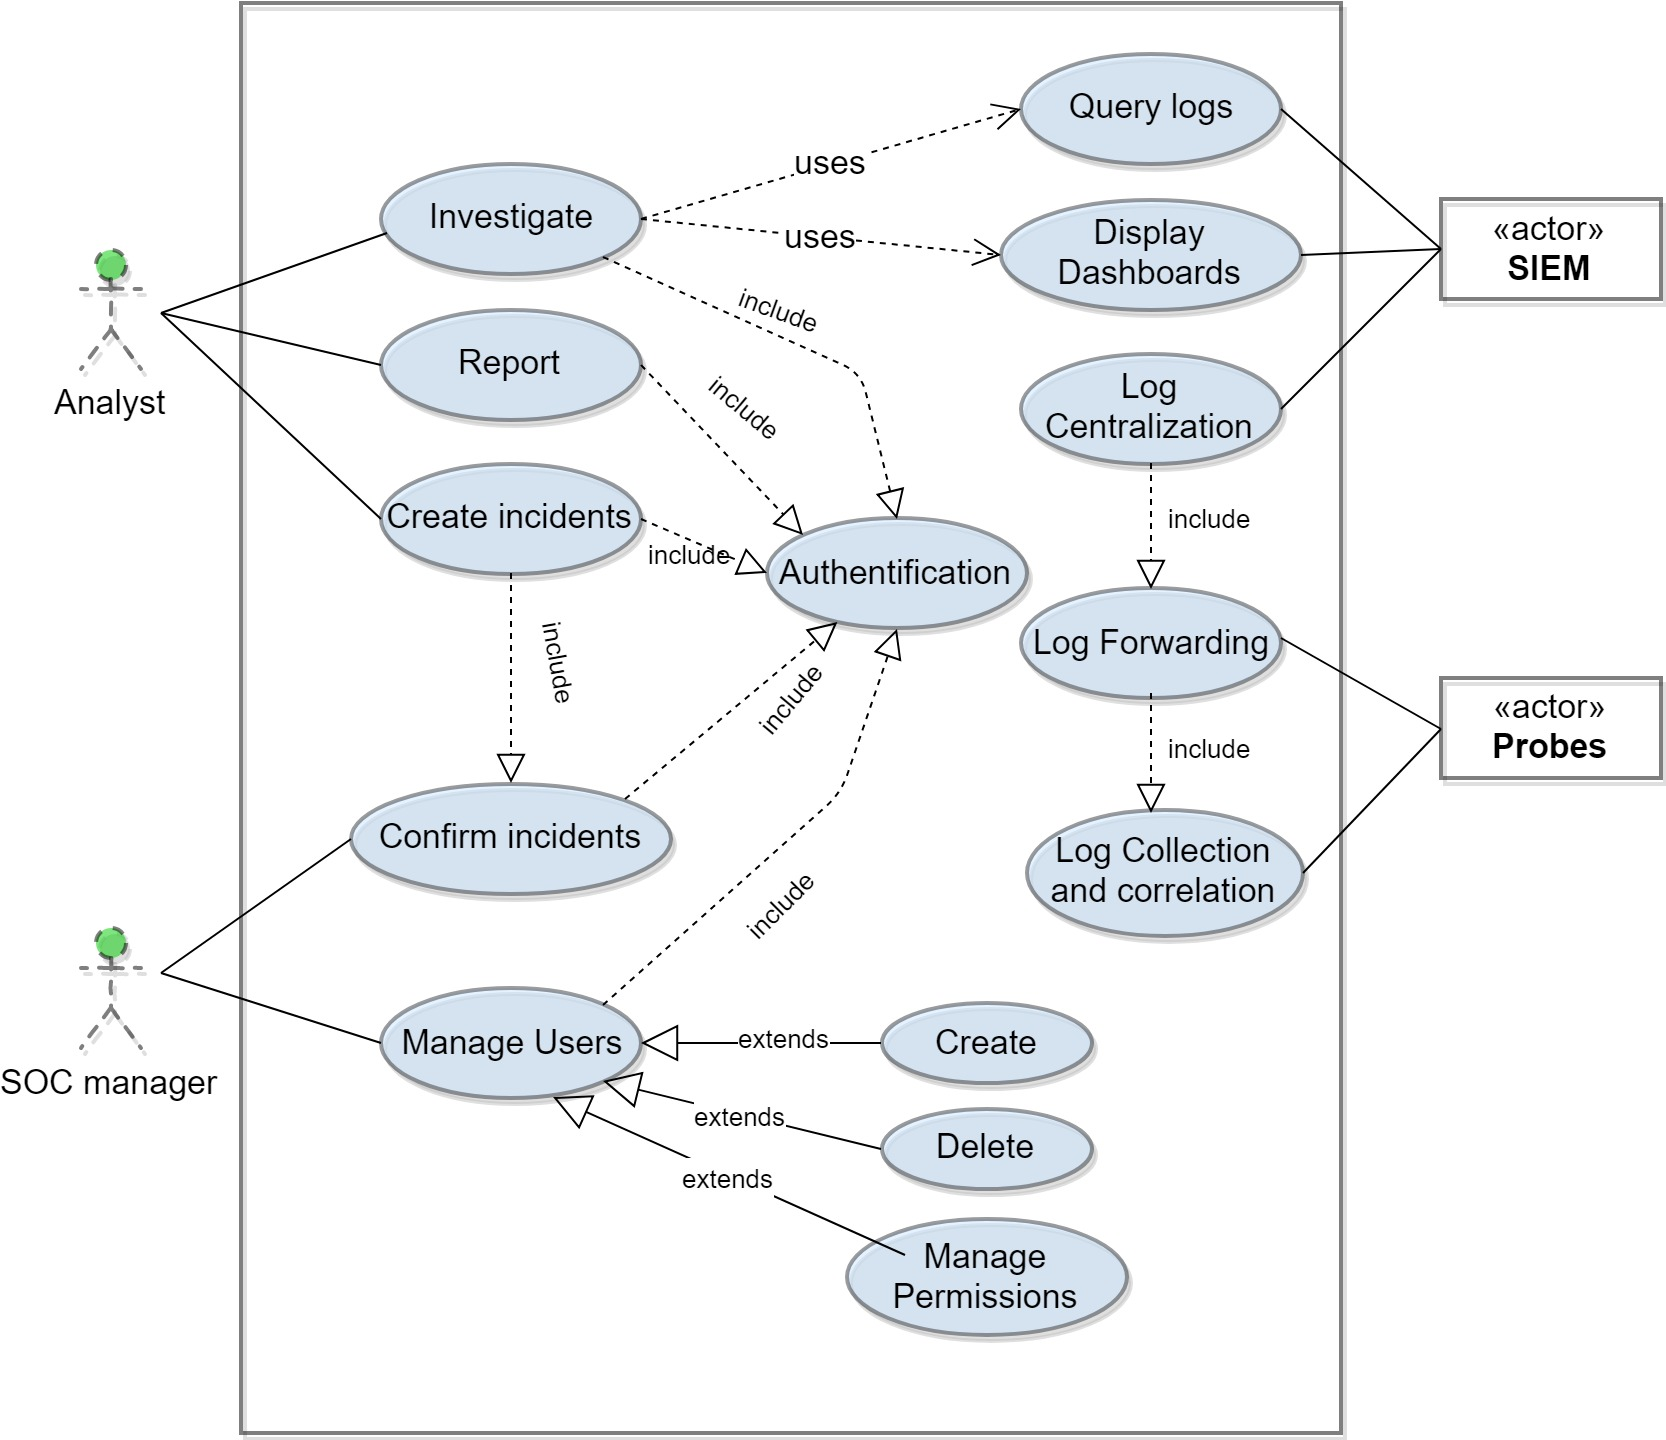
\includegraphics[width=5.5 in]{images/ATHENAusecaseDiagram.jpg}
\caption{System’s General Use Case}
\label{usecase}
\end{center}
\end{figure}  ~

\newpage

The analyst is able to view all logs and alerts through dashboards, the investigation process is accomplished via searching event and querying logs. 
A report must be created by the analyst depending on investigations then he can create incidents if there is an incident by its priority and wait for the SOC manager to confirm that incident.
The Soc manager can also manage users (analysts) and their permissions (which logs or platform to access).

The SIEM (Security information management system) plays a very important role in the system since it is responsible for log's centralization, display and must be efficient and guarantee information's availability and integrity whenever the analyst wants to query logs (old and real-time).

Probes are the main actor that is responsible for collecting and recording logs based on a list of predefined rules and scripts, correlate events and forward logs to the SIEM to prevent disk draining and system failure.

\subsection{Global Sequence Diagram}

In this section, we present the most relevant nominal scenarios in our application using the system sequence diagrams. In a brief description, each system sequence diagram considers one use case at a time and gives the sequence of actions between the user and the system.

\subsubsection *{Nominal scenario for 'Investigation' }

This scenario is illustrated by Figure \ref{seq_diag1}.

In order to start, the authenticated analyst demands summaries for events and alerts in dashboards. The system responds by loading the page, showing multiple dashboards in table, circles, lines and maps. The analyst has the option to filter those dashboards according to different criteria(time, IP address, host name or country name, protocol, port, etc.). 

As a response, the system displays the filtered dashboard. Then, if the analyst notices a malicious activity or a sequence of alerts, he must dug deeper in the details and in some cases extract the PCAP file (A capture file saved in the format that libpcap and WinPcap use can be read by applications that understand that format, such as tcpdump, and in our case Wireshark and NetworkMiner which comes with SecurityOnion) for later examination or proof of breach (for legal use). 

The analyst then creates a report about the incident. In order to do that, he can (if he has permission) access to the treat intelligence platform to see if bro logs indicates or confirm the incident. 

According to its priority, the analyst must create a detailed incident and send it to the SOC manager for confirmation.


\begin{figure}[htbp!]
\begin{center}
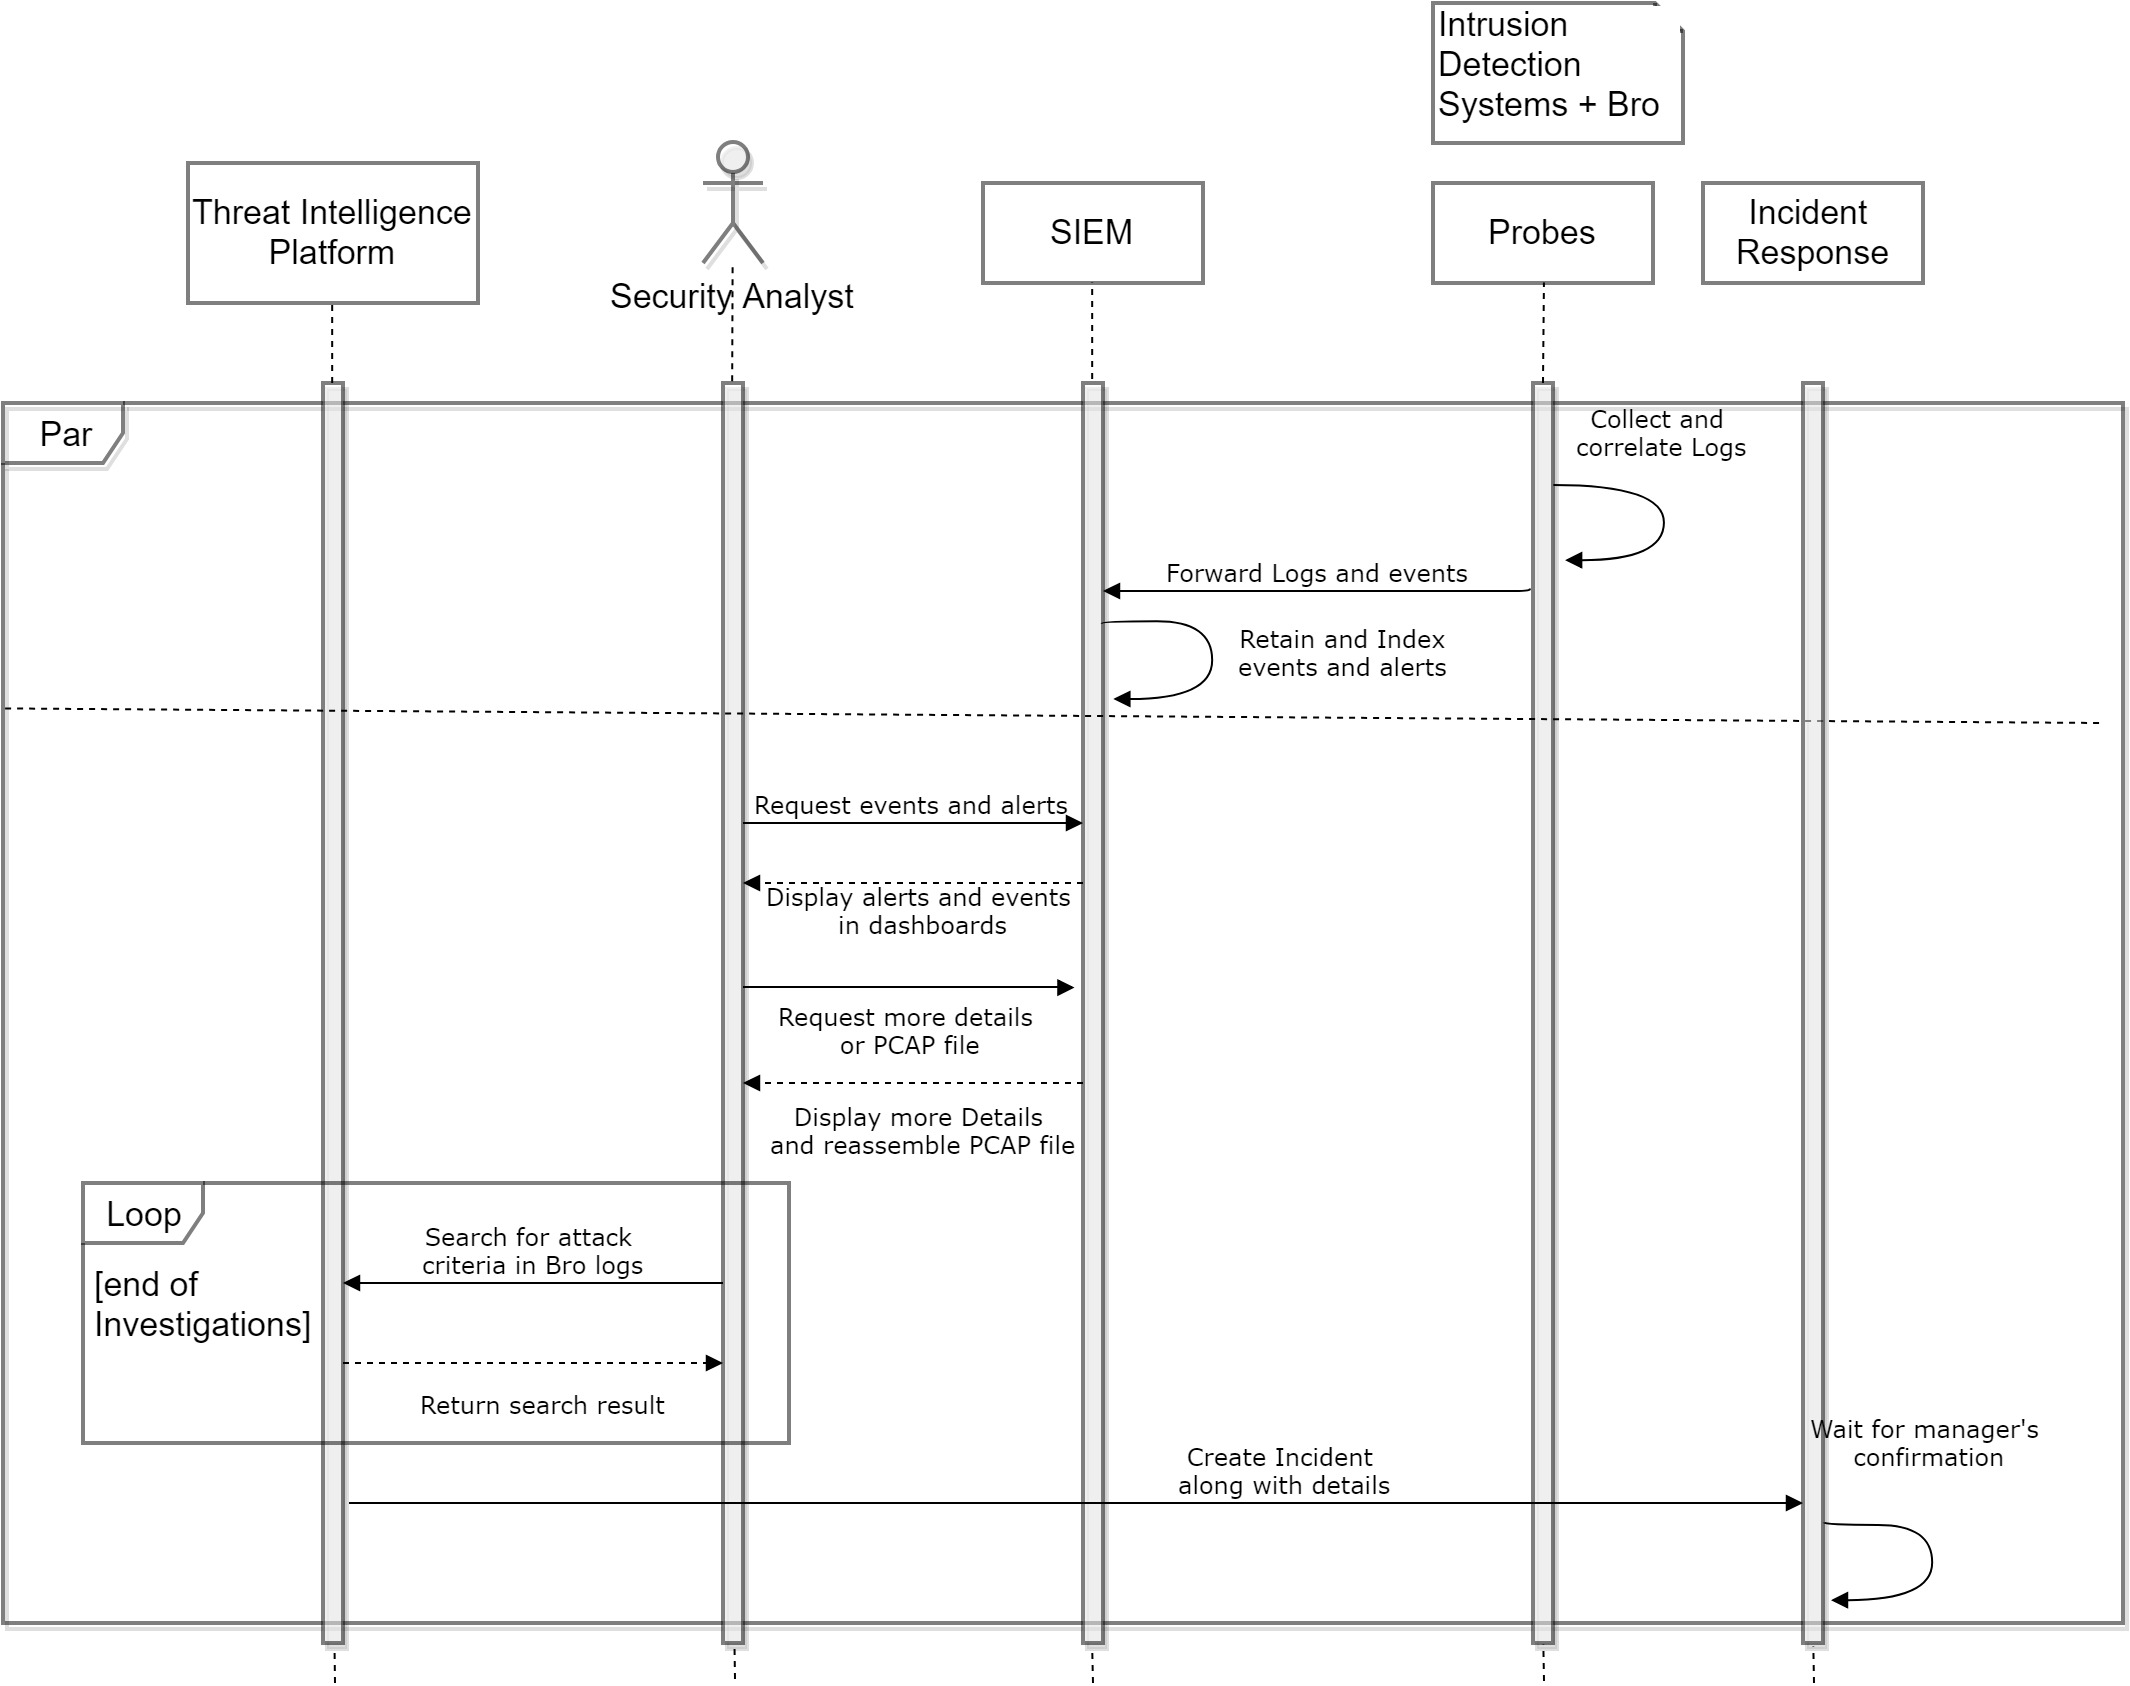
\includegraphics[height=5.0 in]{images/ATHENAGeneralseq.jpg}
\caption{’Investigation’ nominal sequence diagram}
\label{seq_diag1}
\end{center}
\end{figure} 


\subsubsection* {Nominal scenario for 'Incident creation'}

~~~This scenario is illustrated by Figure \ref{seq_diag2}.

The analyst is supposed to run an analyze on bro logs to detect if there is a malicious behaviour or attacks that are undetectable by anti-virus, firewall and even the regular intrusion detection system.

The analyst should have access to the based on local events threat intelligence platform, chooses the time-line(time interval) on which he wishes to run the analyze, the threat intelligence platform then pulls logs and events from the SIEM and index them to fit the pre-configured functions. then display the result in a web page in graphs and tables format. 

Based on those results, the analyst should create the incident report related to that time-line.


\begin{figure}[htbp!]
\begin{center}
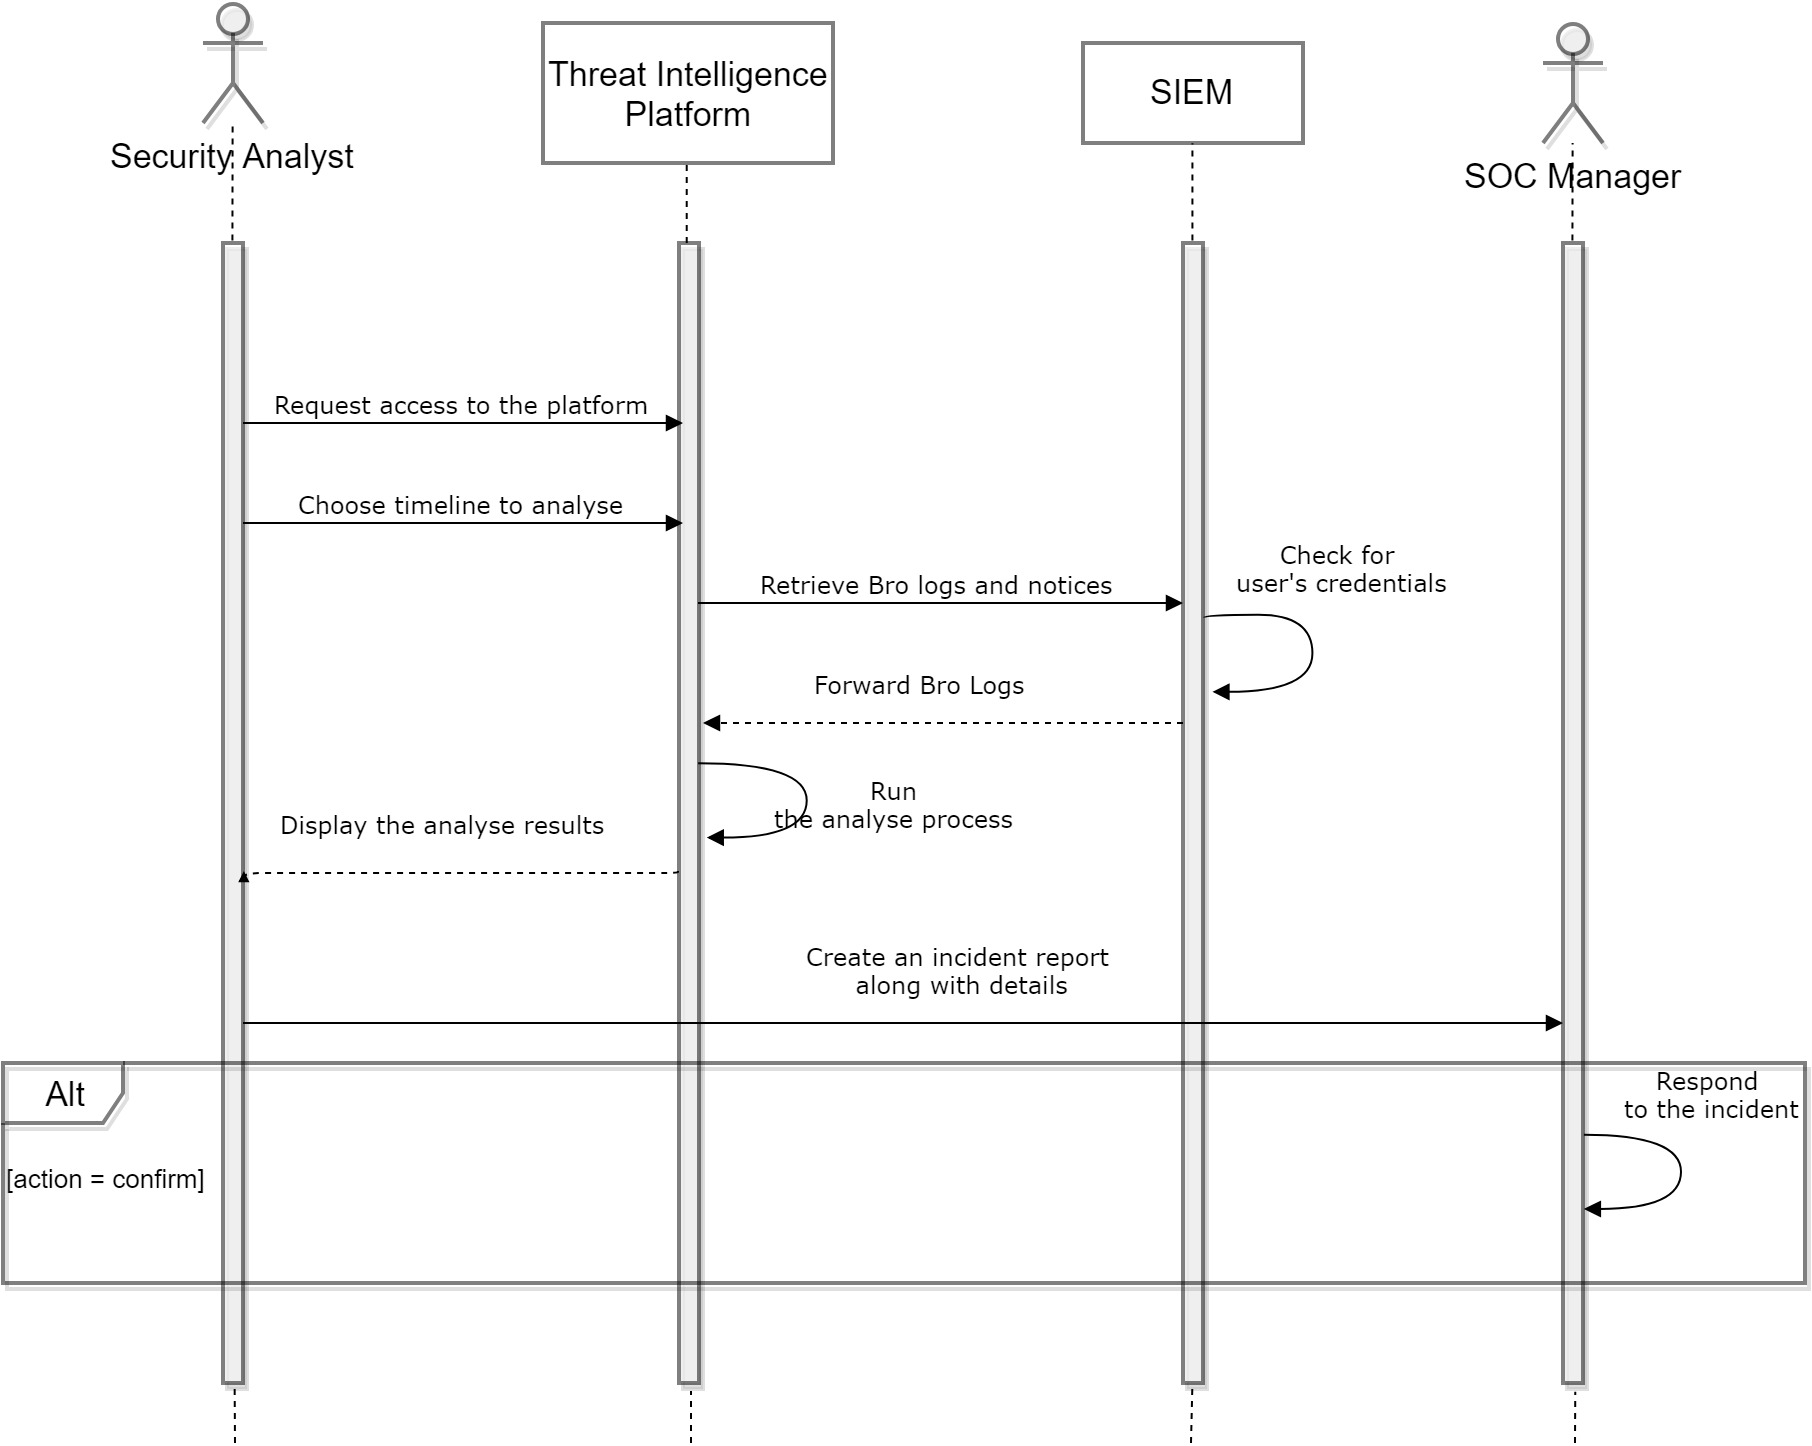
\includegraphics[height=5.0 in]{images/ATHENAThreatintel.jpg}
\caption{’Incident creation’ nominal sequence diagram}
\label{seq_diag2}
\end{center}
\end{figure} 


\subsection *{Conclusion}

Throughout this chapter, we specified and analyzed the requirements that our application should deliver to the future analysts, and we gave the main scenarios and Use Cases of our project. The next chapter aims to go a step further in the process of developing the application via presenting the application’s design.


